%Move from macro to micro, citing from oldest references to the most recent

%What it is: 
%–Overview of previous work in the field 
%– What’s the big picture?
%–Explanation of how your work addresses the gap in the field
%–Enough technical details for the reader to understand your project
%–Explanation of importance/impact of your work 

%What you need to show: 
%–You understand what’s going on in your field, and how your work fits into that. 
%–You have the authority to say your research is important/novel. 

%Can be helpful to... 
%–Restate your hypothesis 
%–Briefly mention an experimental overview (just enough to lead the reader into your Project Plan)

In this section, we will talk about a brief background to Neural Networks and the types of neural networks, leading to the architecture of a Recurrent Neural Network, it's types and it's uses. We will then address some related work in the field of Transit detection, focusing majorly on the vetting. 
\subsection{Neural Networks}
Machine Learning is a type of computer algorithm that is used to predict certain outputs based on the input data. The heuristics of what to learn from the data are automatically identified in the data by this machine learning model in a process called \emph{"Training"}. A supervised machine learning model typically requires a set of inputs and their corresponding actual outputs or labels. The task of the model in the training process is to minimize the difference between the predicted mathematically calculated output it gives based on the certain set of inputs and the actual output, as calculated by a cost function.\\

Deep Learning is a sub-class of Machine Learning which uses mathematical sub-units called neurons. Each of these neurons are arranged in layer like format, where every neuron from one layer is connected to every other neuron in the next layer. The connections between these neurons are called weights, which are multiplicative factors, and each neuron has a bias attached to it, leading to their configuration as
\begin{center}
$a_i = f(W_i * x\textsubscript{i-1} + b_i)$
\end{center}

where $a_i$ is the output of neuron layer \emph{i} when $x\textsubscript{i-1}$ is the input from the previous (\emph{i-1}) layer neurons and the function $f()$ is an activation function which induces non-linearity. Figure below shows a Fully Connected Neural Network or a Multi-layered perceptron. 

%Figure
\begin{figure}[H]
    \centering
    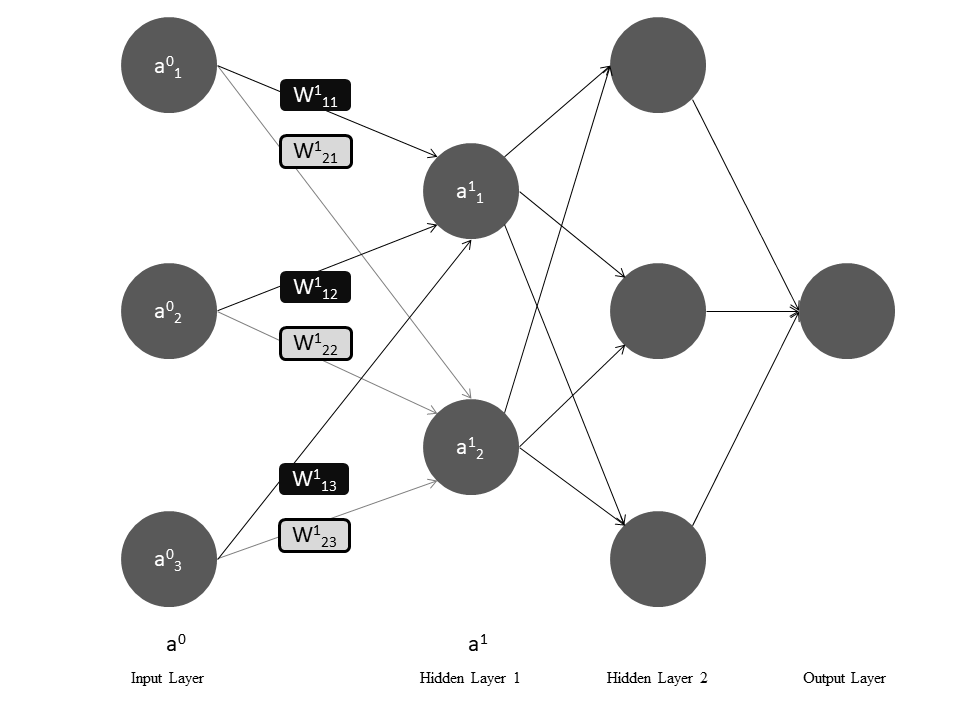
\includegraphics[scale=0.4]{Images/ANN.png}
    \caption{A Fully Connected Neural Network with 2 Hidden Layers. Connections weights are shown between Input layer and Hidden layer 1}
    \label{fig:ANN}
\end{figure}

The \textbf{backpropagation algorithm} changes these weights and biases of the neurons in order to minimize the cost function. Cross Entropy loss is calculated as the cost function for binary classification problems. In order to minimize the cost, we take gradient of the cost (first order derivative) with respect to the parameters of the model and equate it to 0. This indicates the iterative updation of parameters till a minima for the cost is reached, which indicates the optimal model performance.  \\

\textbf{Convolutional Neural Networks} are a class of neural networks which use convolution (or discrete cross-correlation) operation on the input with a kernel/filter at the convolution layer, which is fed to the pooling layer to reduce the dimensionality of the resulting \emph{feature map} by aggregating regions in the neighbouring proximity using mean or maximum values, the output of which is finally fed to a fully connected layer for the prediction of the output. The output of the convolutional layer, or the feature map is given by \\
\begin{center}
    $a_i^{(l)} = f(\sum_{k=1}^K w_i^{(k,l)} * a_{i-1}^{(k)} + b_i^{(l)})$
\end{center}
where the $K$ vectors of length $n_{i-1}$ are input to the $i^{th}$ layer (k=1,2, ..., K) given by $a_{i-1}^{(k)}$, L is the output number of vectors (l=1,2, ...,L) given by $a_i^{(l)}$, $f()$ is the activation function, $*$ is the convolution function, $w_i^{(k,l)}$ is the weight array acting as a filter or kernel and $b_i^{(l)}$ are the bias vector.


\subsection{Recurrent Neural Networks}
Recurrent neural networks are yet another class of NNs which feed the network output back as an input to the network. This allows them to retain information, identify patterns and establish temporal connections, which is suitable for time-series applications.
\begin{figure}[h]
    \centering
    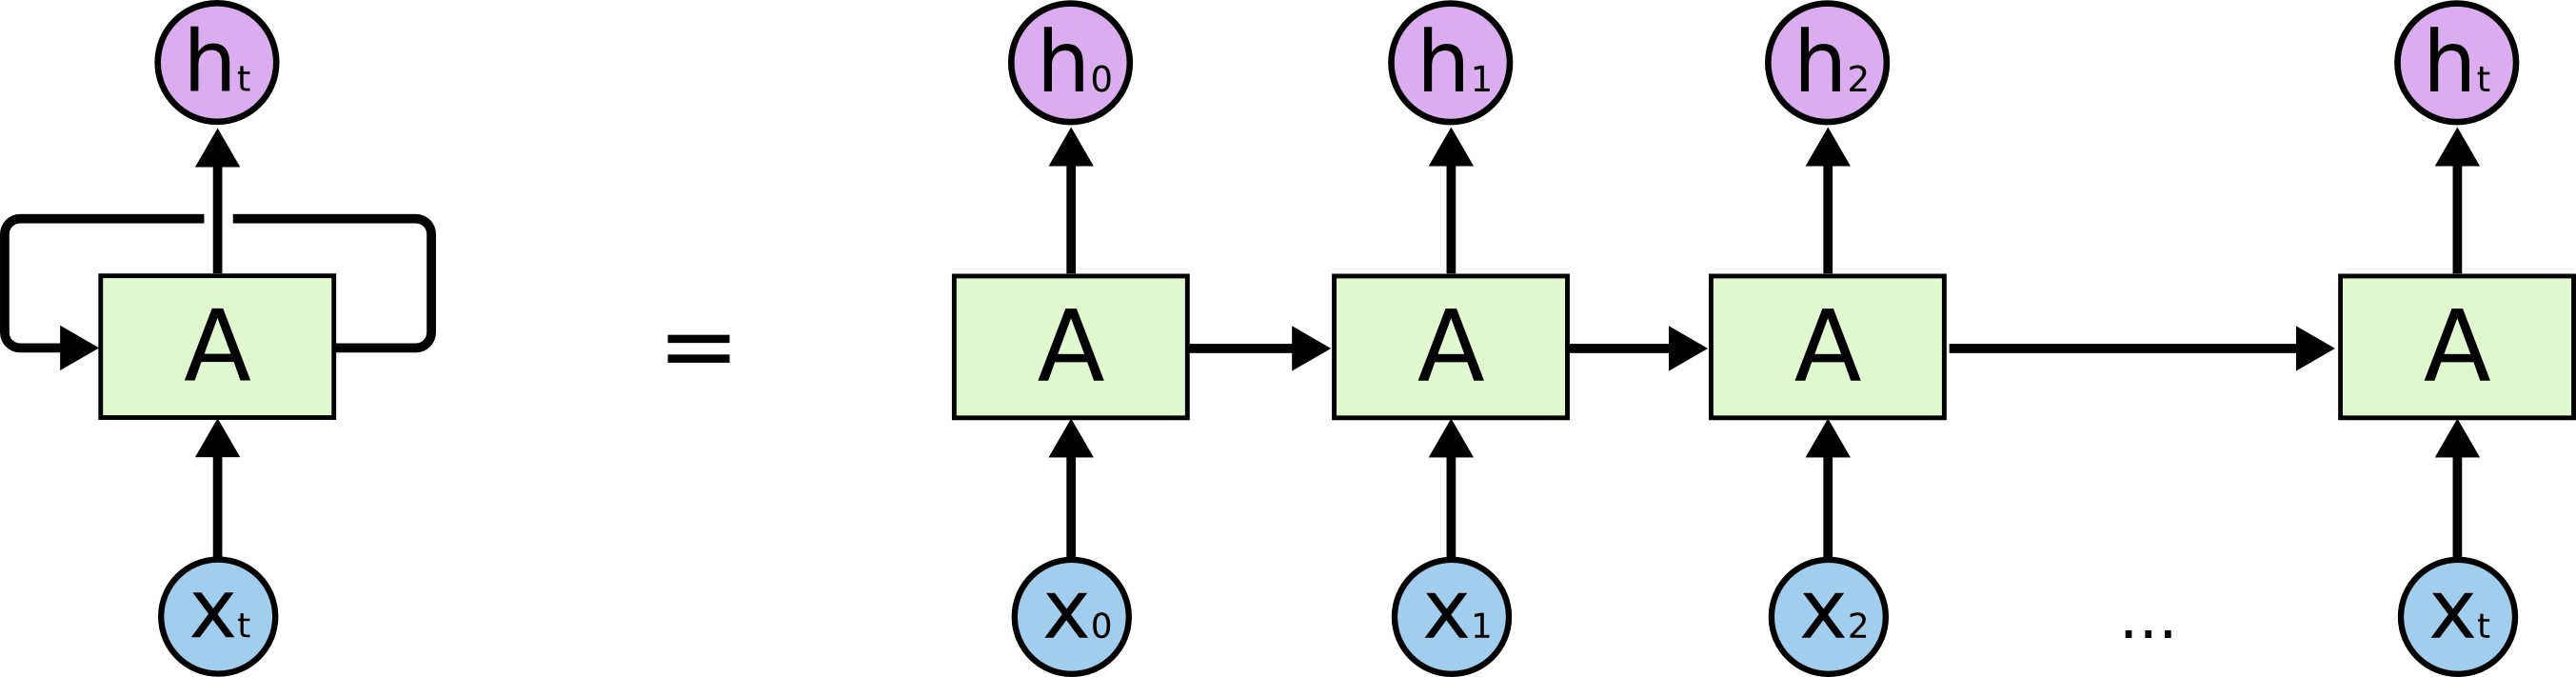
\includegraphics[scale=0.3]{Images/RNNs_1.png}
    \caption{A Recurrent Neural Network. The looped layers are shown unrolled here. \emph{Source}: \href{https://colah.github.io/posts/2015-08-Understanding-LSTMs/}{\textit{Understanding LSTM Networks, Colah 2015}}}
    \label{fig:RNN}
\end{figure}
Long Short Term Memory Networks are a type of gated RNNs that can learn long term dependencies between the data points by removing or adding certain information through the sigmoid gates, controlling this flow of information. There is a Cell-state which flows through the LSTM cells. The information which we need to remove is decided by the first sigmoid gate. The second sigmoid gate in conjecture with $tanh$ of the previous state's output decides what we keep in the cell state. This cell state then factors in with a $tanh$ to the current state's output.
\begin{figure}[h]
    \centering
    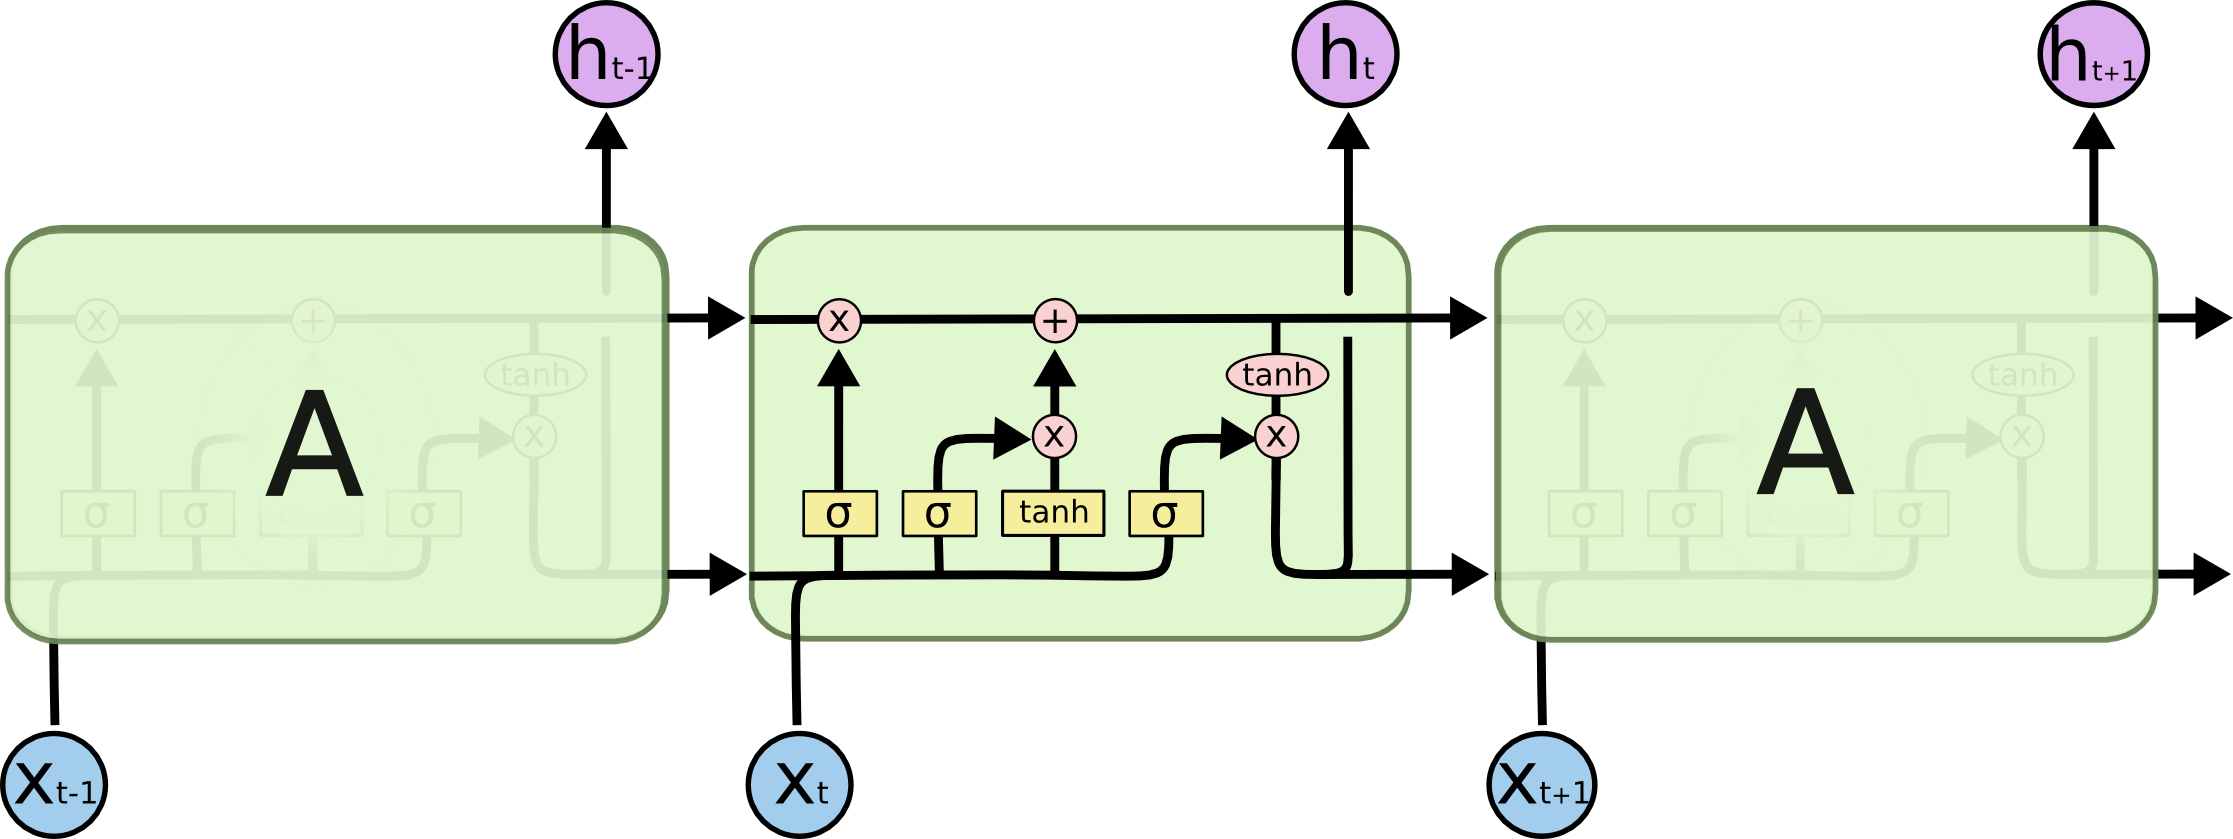
\includegraphics[scale=0.35]{Images/LSTM.png}
    \caption{Simplified architecture of Long Short Term Memory Network. \emph{Source}: \href{https://colah.github.io/posts/2015-08-Understanding-LSTMs/}{\textit{Understanding LSTM Networks, Colah 2015}}}
    \label{fig:LSTM}
\end{figure}
\subsection{Exoplanet Transit Detection}
Transit detection for exoplanets is a field involving space-based high precision photometry. A dip in the stellar flux/brightness indicates a transiting phenomena occuring, or in simpler terms, it indicates the passage of an object between the field of vision from the telescope and the star. We record the stellar brightness over a fixed time span and the resulting flux time series is called a \emph{Light Curve}. The first transit was detected by Charbonneau et al in 1999. 
\begin{figure}[h]
    \centering
    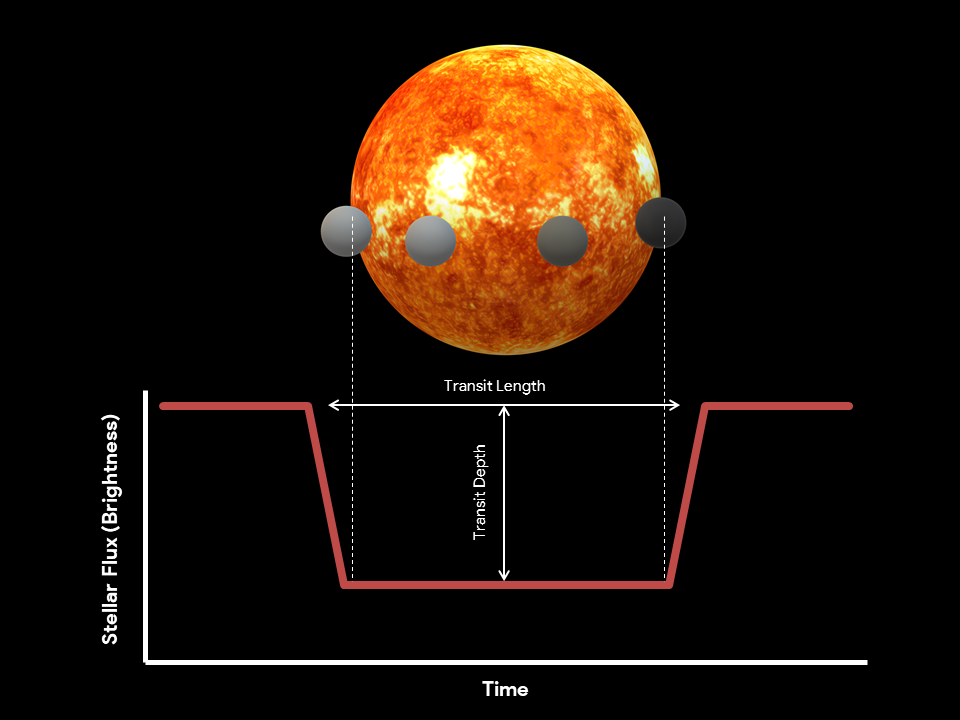
\includegraphics[scale=0.4]{Images/Transit.png}
    \caption{Stellar light curve plotted against a planet transiting it's host star}
    \label{fig:Transit}
\end{figure}

Space based telescope missions, like the Kepler, has a pipeline called \textbf{Science Processing Pipeline} which detects for these transits in noisy data that is collected. The pipeline first calibrates the captured photometric pixels or the TPF (Target Pixel File) over the time span and performs fixed-aperture photometry, and removes instrumental errors. The transits are then detected in the light curves and Threshold Crossing Events (TCEs) are filtered in. The pipeline then classifies each of these TCEs into Kepler's Object of Interests (KOI) based on the light curves. The TCEs can be exoplanet candidates, Astrophysical False Positives (AFP) caused by Eclipsing Binaries (EB) or Background Eclipsing Binaries (BEB), Non Transiting Phenomena (NTP) as caused by starspots, pulsations or stellar flares, or Unknown phenomena (UNKs). The process of classification of the captured light curves into transiting events is called detection while the process of classification of TCEs as a transiting exoplanet is called vetting.\\

Recent advancements for transit detection using deep learning were given by \textbf{Zucker & Giryes} (2018), who proposed a 1D-CNN architecture. They used artificial data created by modelling hypothetical light curves with red noise (or the Brown noise which stimulates the noise produced by Brownian motion processes). \textbf{Pearson
et al.} (2018) used the periodicity of the transit signals in the light curve to fold them on the same phase, enhancing the transit signal. Chintarungruangchai et al. (2018) used a 2D-CNN architecture with phase folding to demonstrate state of the art performance for transit detections.

Several automatic vetters have emerged in the past years to deal with large amounts of data and reduce manual vetting effort. Kepler pipeline uses Robovetter and Autovetter for classifying the transits as planet candidates. Robovetter or Robotic Vetting process defined by Coughlin et al. is a Decision Tree which replicates the manual steps taken while vetting the TCEs as a series of if-else statements. A "innocent until proven guilty" approach is followed to maximize the recall for detecting planet candidates. The robovetter uses a phased light curve which is detrended using least squares method, leaving the in-transit points when detrending, thereby preserve the transiting events when detrending the light curve. The decisions making process involves checking any secondary identified eclipsing binary from another system, checking transit shape and filtering out eclipsing binaries, and checking for centroid shifts and ephimeris match to other TCEs and variable stars in Kepler field. Robovetter classifies the final output as a planet candidate or a non planet-candidate. Autovetter, on the other hand, is a Machine Learning model which uses random forests. Random forests are ensembles of decision trees, where each tree tests a set of random vector of attributes (real random variables) and each tree have branches based on binary classifications of these attributes, terminating at leaf nodes which gives the individual decisions of these trees. A whole classification is taken based on maximum votes from the individual tress. Autovetter classifies the transit event as PC, AFP or NTP.

\subsubsection{Astronet}
Shallue and Vanderburg in 2018 proposed a Deep Learning method for classification of transit events as Planetary candidates or non planetary candidates. They used a disjoint 1D Convolutional Neural Network for the classification, where the two convolutional columns incorporate a global view and a local view of the transit. They use basis spline to flatten the light curves after isolating the transits and interpolating the isolated portions linearly, and dividing it by the best-fit spline. The TCE light curve is then folded and binned into a 1 Dimensional vector. The bin width, $\delta$ is taken $> \lambda$ to overlap the bins and minimize scattering. The global view uses a fix $\lambda$, which is a fraction of overall TCE period and hence is common for all light curves and results in 2,001 points of time, while the local view uses a $\lambda$ as a fraction of TCE duration, making it unique to each transit, giving a local transit and resulting in 201 points of time. The global and local view convolution columns (having local pooling layers internally) are fed into a fully connected layer which has a final sigmoid neuron, describing the probability of the transit to be a planet or not (1 and 0 respectively).\\

Shallue and Vanderburg (2018) reports an accuracy of 95.8\% and an average precision of 95.5\% with Q1-Q17 Data Release 24.


\subsubsection{Exonet}
Ansdell et al (2018) improves on the accuracy of Astronet by introducing scientific domain data for transit classification. The key improvements of Exonet are:
\begin{itemize}
    \item They used a light Centroid time series (Centroid Curves). The centroid displacement is calculated from the TPF center and then a similar data pre-processing as light curves, involving flattening, phase folding and creating local and global views, is followed. The centroid curve is normalized over its standard deviation and median, and  is presented as an input to the model
    \item They used Stellar parameters such as star's effective temperature ($T_{eff}$), surface gravity (log $g$), stellar metallicity ($[Fe/H]$), radius ($R_{*}$), mass ($M_*$) and density ($\rho_*$), as an input to the fully connected layers for classification
    \item A different method ($LSQUnivariateSpline$ from $scipy$) for spline fitting was used as compared to Astronet ($bspline$ from $PyDL$) resulting in faster (upto 5X) data processing times.
    \item In addition to flipping of time series in light curves for data augmentation, addition of random Gaussian noise was also used. Also, both these data augmentation techniques were also used for centroid curves.
\end{itemize}
They also created a reduced architecture for Exonet and Astronet, called Exonet-XS and Astronet-XS respectively, where the model size and parameters were reduced significantly and usage of a global pooling layer instead of local pooling layers, which resulted in a very small drop of accuracy from the original models. They report an accuracy of 97.5\% and an average precesion of 98.0\% for Exonet, which is an improvement of 1.7\% and 2.5\% increase from astronet, and is the current state of the art. Exonet-XS reports an accuracy of 96.6\% and an average precision of 96.3\%. Figure 2.5 shows the model architecture for Exonet, Astronet and their reduced XS models.
\begin{figure}[H]
    \centering
    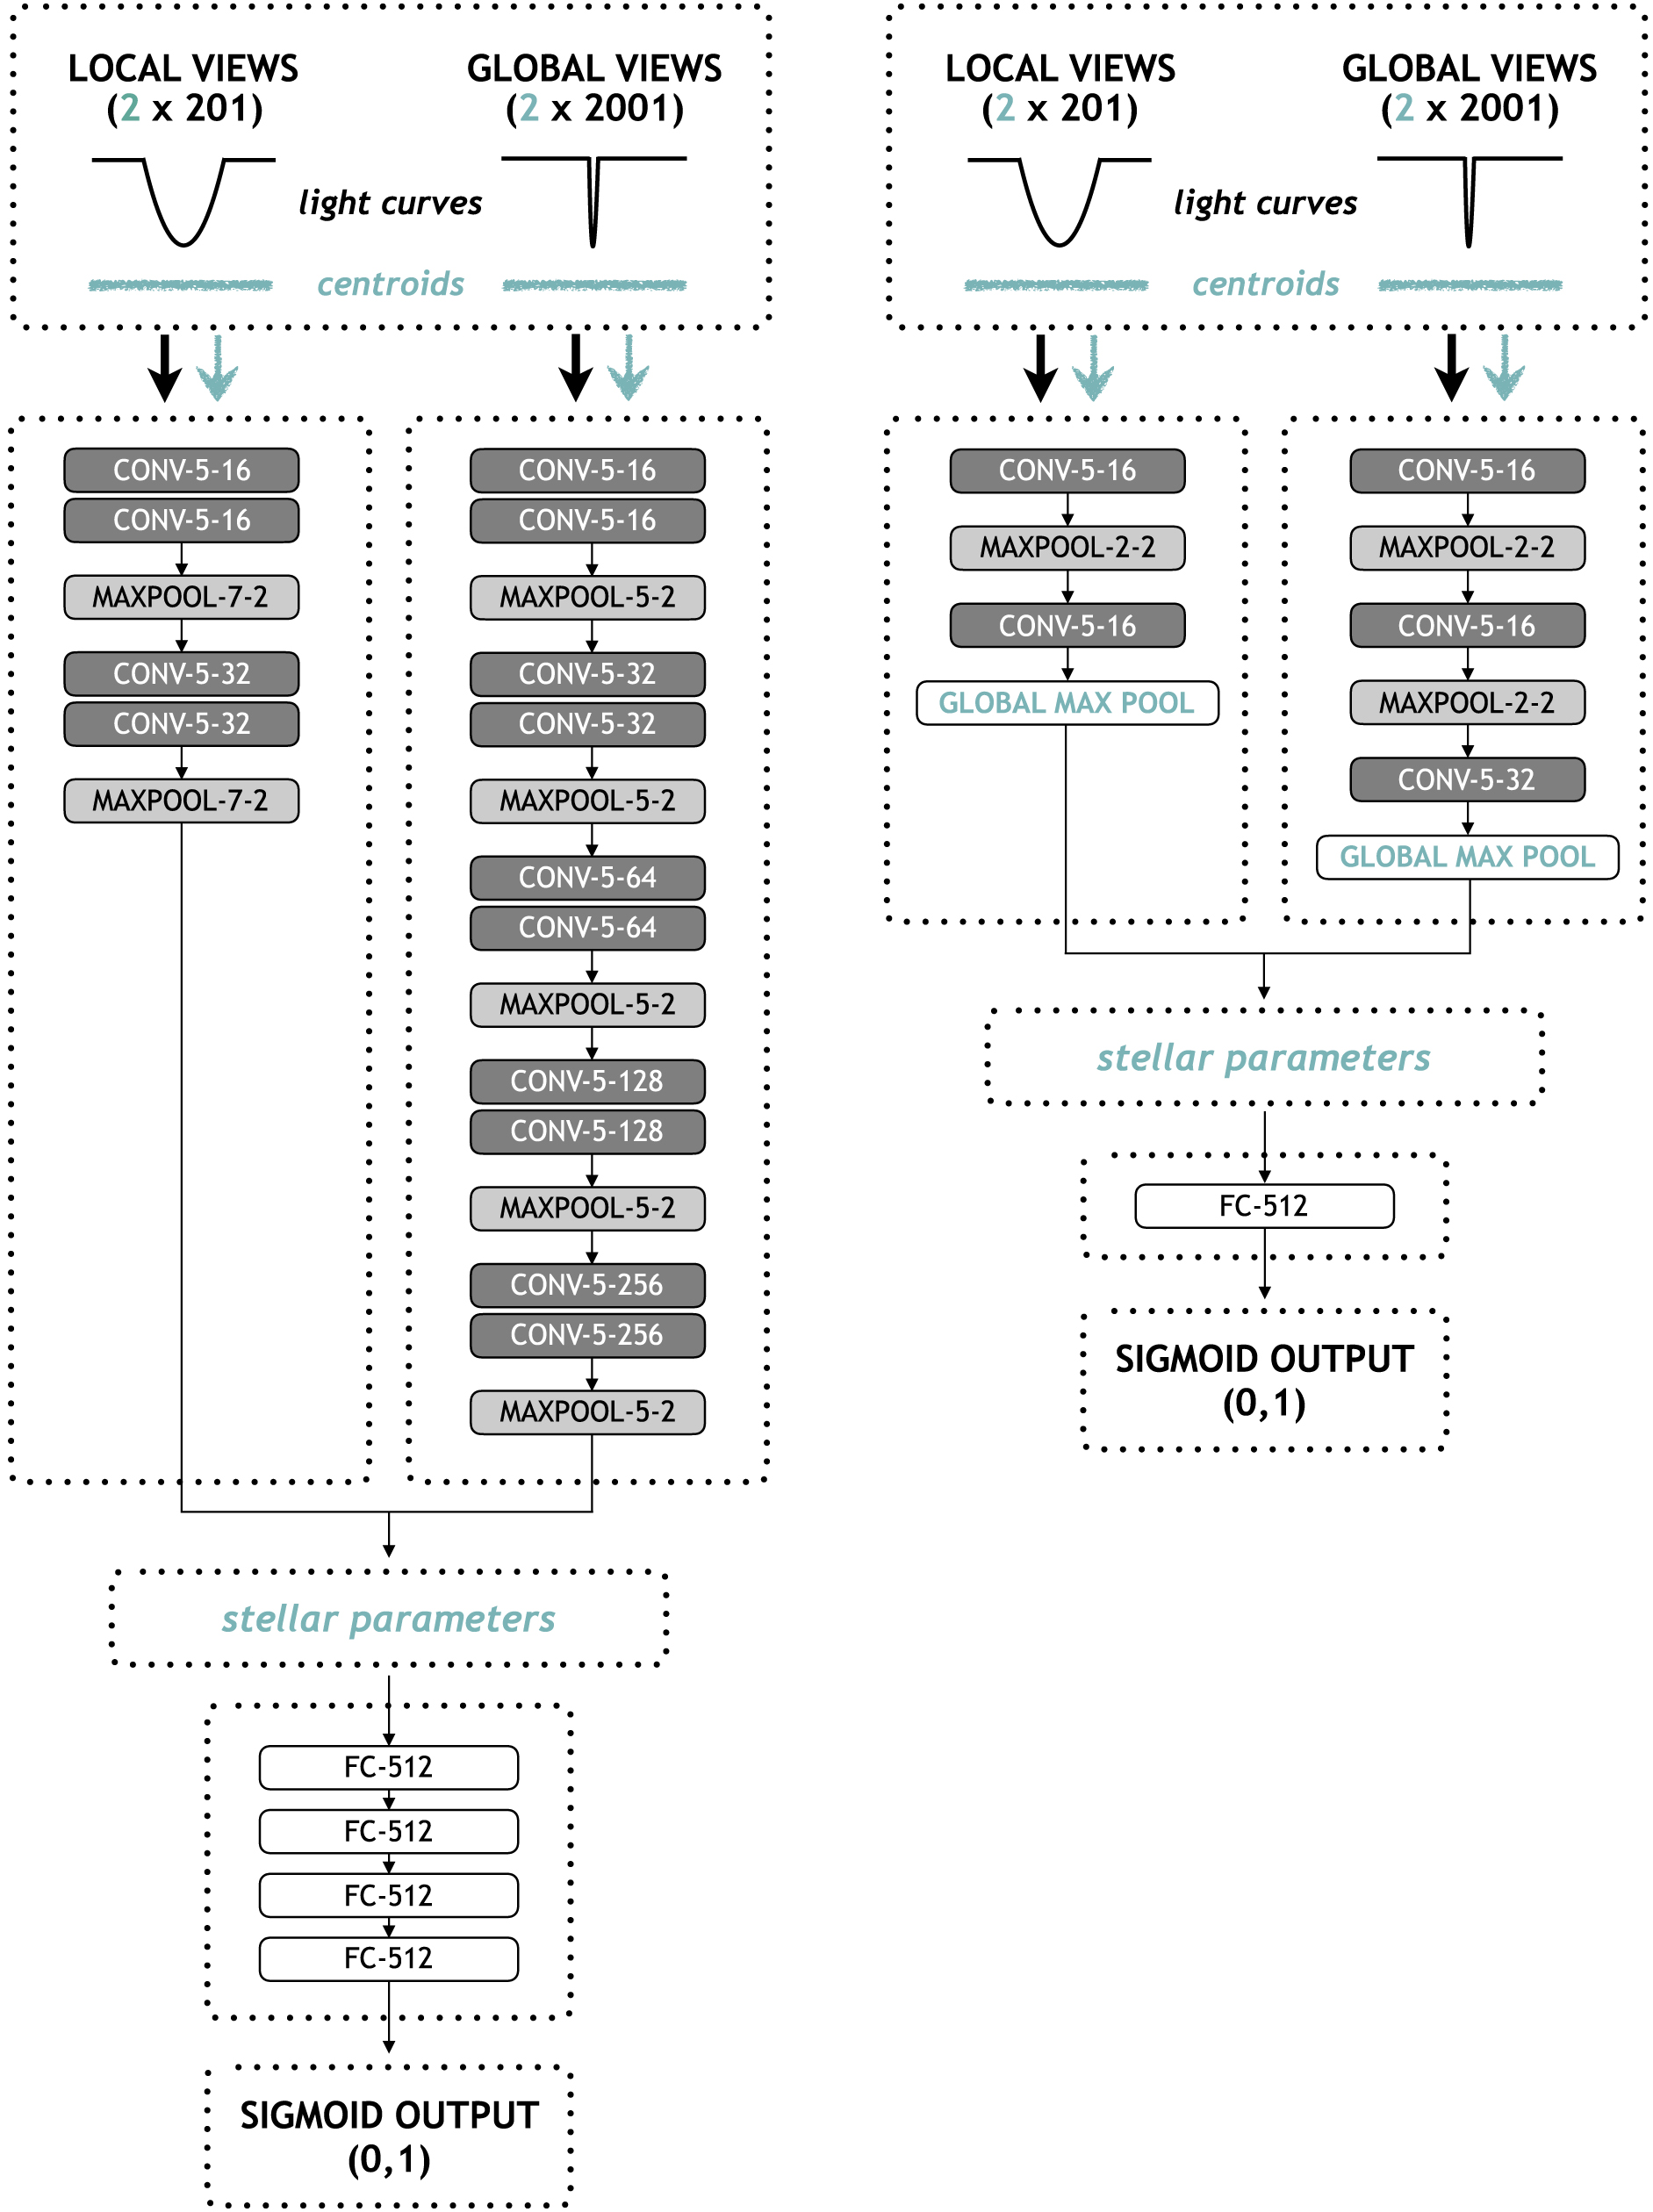
\includegraphics[scale=0.5]{Images/Ansdell.jpg}
    \caption{Exonet model additions are shown in Blue over the backbone Astronet model on the left while reduced XS models are shown on the right. The convolutional layers are denoted as CONV-〈kernel size〉-〈number of feature maps〉, the max pooling layers are denoted as MAXPOOL-〈window length〉-〈stride length〉, and the fully connected layers are denotedas FC-〈number of units〉. Source: Ansdell et al. (2018)}
    \label{fig:Ansdell}
\end{figure}